\documentclass[10pt,a4paper]{article}
\usepackage[utf8]{inputenc}
\usepackage[english]{babel}
\usepackage{amsmath}
\usepackage{amsfonts}
\usepackage{amssymb}
\usepackage{graphicx}
%\usepackage{fourier}
\usepackage[left=2cm,right=2cm,top=2cm,bottom=2cm]{geometry}

\usepackage{float}
\newcommand*\Laplace{\mathop{}\!\mathbin\bigtriangleup}

\author{Sven Karsten}
\title{Deriving the Navier-Stokes equations}


\newcommand{\e}{\mathrm{e}}
\renewcommand{\d}{\mathrm{d}}
%\renewcommand{\vec}[1]{\mathbf{#1}}

\usepackage{empheq}
\newcommand*\widefbox[1]{\fbox{\hspace{2em}#1\hspace{2em}}}

\begin{document}

\maketitle

\tableofcontents

\section{Forces acting on a fluid}

\subsection{Newton's second law of motion}

Newton's second law of motion:

\begin{align}
\vec{F} = m \vec{a}
\end{align}

For a theoretical physicist more reasonable form 
%
\begin{align}
\vec{a} = \frac{\d^2 \vec{r}}{\d t^2} = \frac{\vec{F}}{m} 
\end{align}
%
from that one can calculate $\vec{r}(t)$ and $\vec{u}(t)={\d \vec{r}}/{\d t}$ for all times $t$.


\subsection{Fluid parcels}

For the sake of simplicity we restrict ourselves to a two-dimensional fluid.
%
Consider a fluid parcel with a center of mass located at $(x,y)$ at time $t$ with mass $\Delta m = \rho(x,y,t) \Delta x \Delta y $.
%
The extent (volume) $\Delta x \Delta y$ of the parcel shall be so small that its location can be described only by the center of mass, but large enough to contain so many molecules that it can be treated as continuum.
%
Further we assume that the mass $\Delta m$ is constant over time, such that, in principle, its extent (volume) could change in time, i.e. $\Delta x \Delta y=\Delta x(t) \Delta y(t)$, if the density $\rho(x,y,t)$ is time-dependent.
%
However, we will skip the time arguments in the following for the sake of brevity. 

The dynamics of such a parcel is determined by the acceleration vector $\vec{a}(x,y,t) $ that is given by the forces acting on it.
%
In the following we want to model each of these forces from reasonable assumptions.


\subsection{Body forces}

\begin{figure}[H]
\begin{center}
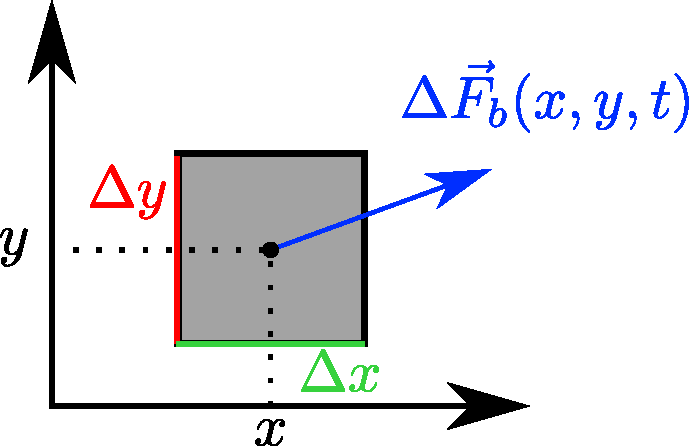
\includegraphics[scale=0.7]{body_forces.pdf}
\end{center}
\end{figure}
%
Assume the fluid parcel to be so small that body forces act effectively only on center of mass $(x,y)$ then the accelerated due to theses forces as
%
\begin{align}
\vec{a}^b(x,y,t) = \frac{\Delta \vec{F}^b(x,y,t)}{\Delta m} = \frac{\Delta \vec{F}^b(x,y,t)}{\rho(x,y,t)\Delta x \Delta y} 
\end{align}
%
If we write $\vec{r} = (x,y)$ and define $\vec{f}^b(\vec{r},t)={\Delta \vec{F}^b(\vec{r},t)}/{\rho(\vec{r},t)\Delta x \Delta y}$ as the body force density we can write down for acceleration due to body forces as
%
\begin{align}
\boxed{
\vec{a}^b(\vec{r},t) =  \frac{\vec{f}^b(\vec{r},t)}{\rho(\vec{r},t)}
}
\end{align}
%

\subsection{Repelling forces (pressure)}

\begin{figure}[H]
\begin{center}
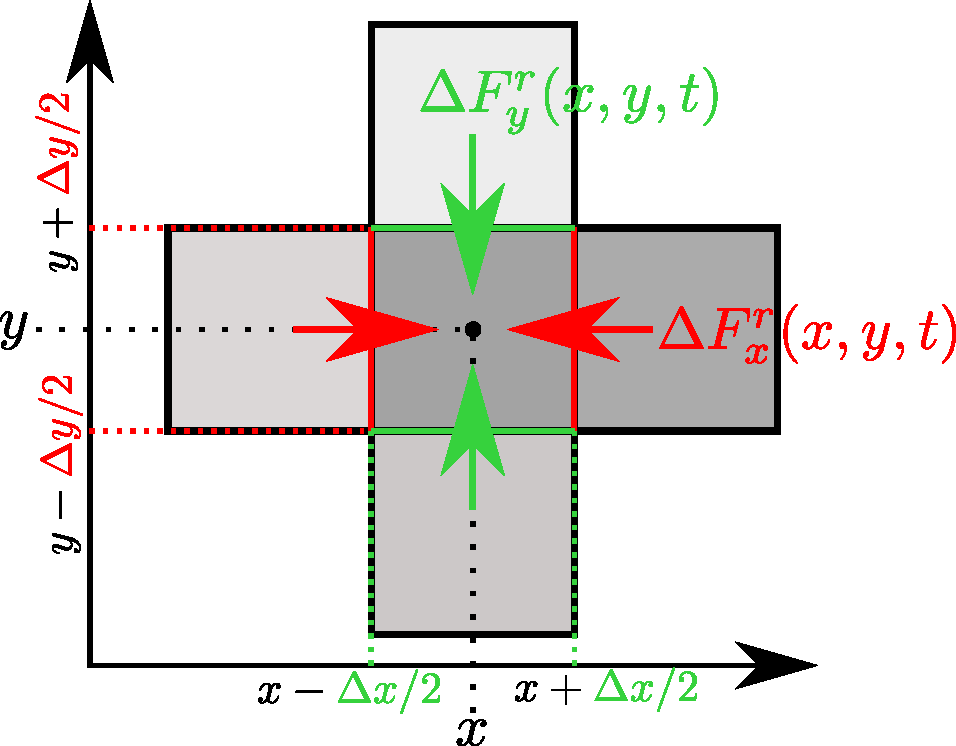
\includegraphics[scale=0.7]{repelling_forces.pdf}
\end{center}
\end{figure}
%
If the repelling force is due to collisions of the molecules from one parcel to another, the force in $x$-direction should be proportional to shared area $\Delta y$ of the parcels.
%
If we call the proportionality factor that takes these collisions macroscopically into account $p(x,y,t)$, then the total force in $x$-direction is
%
\begin{align}
\Delta F^r_x(x,y,t) = p(x-\Delta x/2, y, t) \Delta y - p(x+\Delta x/2, y, t)\Delta y
\end{align}
%
The resulting acceleration in $x$-direction is then
%
\begin{align}
a_x^r(x,y,t) = \frac{\Delta F^r_x(x,y,t)}{\rho(x,y,t) \Delta x \Delta y} = \frac{1}{\rho(x,y,t)} \frac{ p(x-\Delta x/2, y, t)  - p(x+\Delta x/2, y, t)}{\Delta x}
\end{align}
%
If we let $\Delta x \to 0$ we obtain with the definition of the partial derivative
%
\begin{align}
a^r_x(x,y,t) =  -\frac{1}{\rho(x,y,t)} \frac{ \partial p(x, y, t)}{ \partial x}
\end{align}
%
The very same line of reasoning can be done for the repelling forces in $y$-direction.

Introducing the Nabla vector operator as
%
\begin{align}
\nabla := \begin{pmatrix}
\frac{\partial}{\partial x} \\
\frac{\partial}{\partial y}
\end{pmatrix}
\end{align}
%
the acceleration vector stemming from the repelling forces can be written down as
%
\begin{align}
\boxed{
\vec{a}^r(\vec{r},t) =  -\frac{1}{\rho(\vec{r},t)} \nabla p(\vec{r}, t)
}
\end{align}
%

\subsection{Attracting forces (friction)}

\begin{figure}[H]
\begin{center}
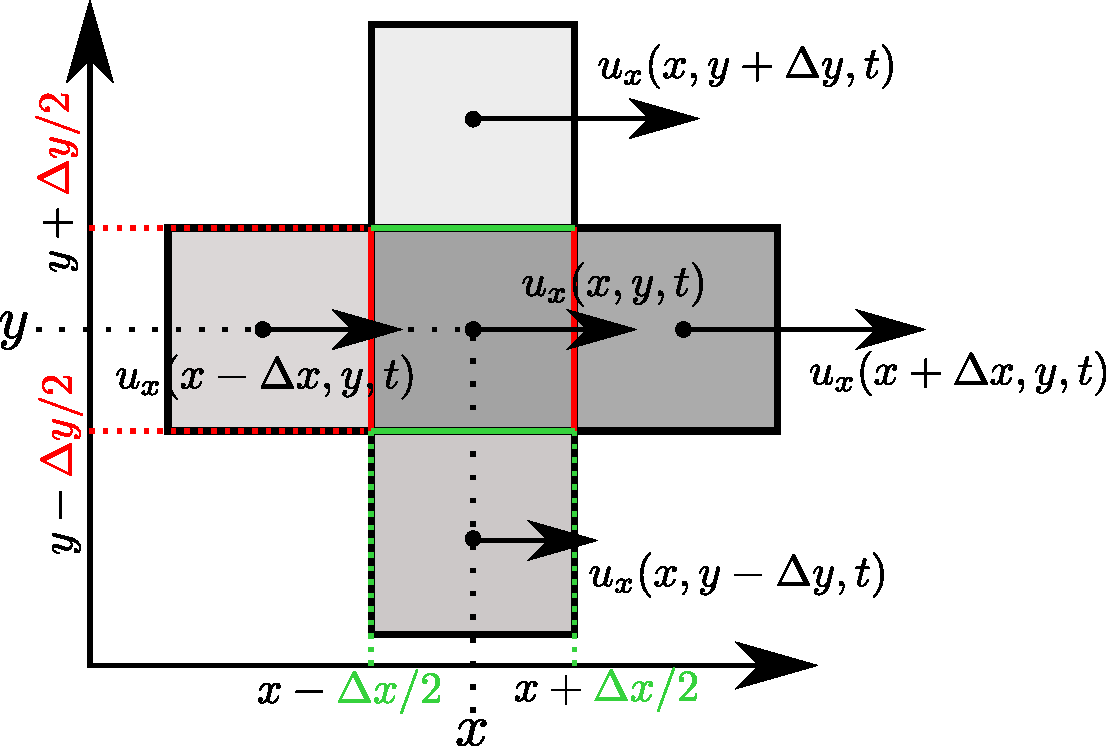
\includegraphics[scale=0.7]{attracting_forces.pdf}
\end{center}
\end{figure}
%
The molecules inside the different parcels do not only repel each other but they are also held together by attracting forces if they are not coming too close.
%
One can imagine that if neighboring parcels have different velocities, these forces act against the difference.
%
Moreover, it is reasonable to assume that the force on the center of mass grows with the contact surface and shrinks with the distance to these boundaries.
%
If we restrict our selves first to the attracting force $\Delta F^a_{x, y}$ in $x$-direction from the parcels above and below (indicated by the additional index $y$) our central parcel, one can then write
%
\begin{align}
\Delta F^a_{x, y} & =   \nu(x, y+\Delta y/2, t) \frac{\Delta x}{\Delta y} [u_x(x, y+\Delta y, t) - u_x(x, y, t)] \\
& - \nu(x, y-\Delta y/2, t) \frac{\Delta x}{\Delta y} [u_x(x, y, t)-u_x(x, y-\Delta y, t)] 
\end{align}
%
where we introduced the macroscopic proportionality factor $\nu(x,y,t)$ that is determined by the molecular properties of the fluid.
%
On top we assumed that the force only linearly depends on the velocity difference, however, there is no reason (apart from simplicity) that higher orders should not play a role.

Now we consider the corresponding acceleration
%
\begin{align}
a^a_{x, y} = \frac{\Delta F^a_{x, y}}{\rho(x,y,t)\Delta x \Delta y}  = \frac{1}{\rho(x,y,t)}  & \left \{ \frac{\nu(x, y+\Delta y/2, t)}{\Delta y}    \frac{u_x(x, y+\Delta y, t) - u_x(x, y, t)}{\Delta y} \right. \\
& \left. -  \frac{\nu(x, y-\Delta y/2, t)}{\Delta y} \frac{u_x(x, y, t)-u_x(x, y-\Delta y, t)}{\Delta y} \right\},
\end{align}
%
In order to get a proper expression for it we first make use of the properties of our fluid parcels, i.e. that it can be treated as a point particle without inner structure but with finite extent and thus all properties are constant inside of the parcel.
%
Hence we can equal
%
\begin{align}
u_x(x, y+\Delta y, t) = u_x(x, y+3 \Delta y/2, t) \\
u_x(x, y, t) = u_x(x, y+\Delta y/2, t) \\
u_x(x, y-\Delta y, t) = u_x(x, y-\Delta y/2, t) 
\end{align}
%
Second we decrease $\Delta y$ so far that we can well approximate (with the definition of the partial derivative)
%
\begin{align}
 \frac{u_x(x, y+3\Delta y/2, t) - u_x(x, y+\Delta y/2, t)}{\Delta y} \approx \left. \frac{\partial u_x(x, y', t)}{\partial y'} \right |_{y'=y+\Delta y/2} \\
 \frac{u_x(x, y+\Delta y/2, t)-u_x(x, y-\Delta y/2, t)}{\Delta y} \approx \left. \frac{\partial u_x(x, y', t)}{\partial y'} \right |_{y'=y-\Delta y/2}
\end{align}
%
which becomes exact in the limit $\Delta y \to 0$.
%
Inserted in the equation for the acceleration this leads to
%
\begin{align}
a^a_{x, y}  = \frac{1}{\rho(x,y,t)}  & \left \{ \frac{\nu(x, y+\Delta y/2, t)}{\Delta y}    \left. \frac{\partial u_x(x, y', t)}{\partial y'} \right |_{y'=y+\Delta y/2} -  \frac{\nu(x, y-\Delta y/2, t)}{\Delta y} \left. \frac{\partial u_x(x, y', t)}{\partial y'} \right |_{y'=y-\Delta y/2} \right\}
\end{align}
%
Now we recognize again the definition of the partial derivative and can finally perform the limit $\Delta y \to 0$ explicitly and obtain
%
\begin{align}
 a^a_{x, y}  = \frac{1}{\rho(x,y,t)} \frac{\partial}{\partial y} \left( \nu(x,y,t) \frac{\partial u_x(x, y, t)}{\partial y} \right) 
\end{align}
%
As a good approximation one can assume that the factor $\nu(x,y,t)$, i.e. the dynamic viscosity is constant in time and space.
%
Then the expression for this component of the acceleration in $x$-direction simplifies to
%
%
\begin{align}
a^a_{x, y}  = \frac{\nu}{\rho(x,y,t)} \frac{\partial^2 u_x(x, y, t)}{\partial y^2}  .
\end{align}

The very same line of reasoning can be applied for the forces that act in $x$-direction stemming from the parcels that are located to the left and right of the central parcel.
%
This yields the acceleration component $\Delta a^a_{x, x} $ and adding this up to $\Delta a^a_{x, y}$ we obtain the full acceleration in $x$-direction as 
%
\begin{align}
a^a_{x}  = \frac{\nu}{\rho(x,y,t)} \left[ \frac{\partial^2 u_x(x, y, t)}{\partial y^2} + \frac{\partial^2 u_x(x, y, t)}{\partial x^2} \right] = \frac{\nu}{\rho(x,y,t)} \Laplace u_x(x, y, t) ,
\end{align}
%
where we have introduced the Laplace operator is $\Laplace = \partial^2/\partial x^2 + \partial^2/\partial y^2$ in two dimensions and would have an additional summand accounting for $z$ in three dimensions.

If we perform the same consideration for the forces in $y$-direction we would get 
%
\begin{align}
a^a_{y}  = \frac{\nu}{\rho(x,y,t)} \Laplace u_y(x, y, t) .
\end{align}
%
Thus in compact vector notation we obtain for the acceleration of our parcel at $x,y,t$ due to friction/viscosity forces
%
\begin{align}
\boxed{ \vec{a}^a(\vec{r},t)  = \frac{\nu}{\rho(\vec{r},t)} \Laplace \vec{u}(\vec{r}, t)} .
\end{align}
%

\section{Equations of motion in a rotating system}

It is important to know that Newton's laws are only applicable in inertial systems described by Cartesian coordinates.
%
However, we are often in the situation that we want use other coordinate systems that are better suited for the given situation.

Assume we have two systems, where $\Sigma$ should be an inertial system and $\Sigma'$ should be rotating anti-clockwise against $\Sigma$ with constant angular velocity $\omega$.
%
\begin{figure}[H]
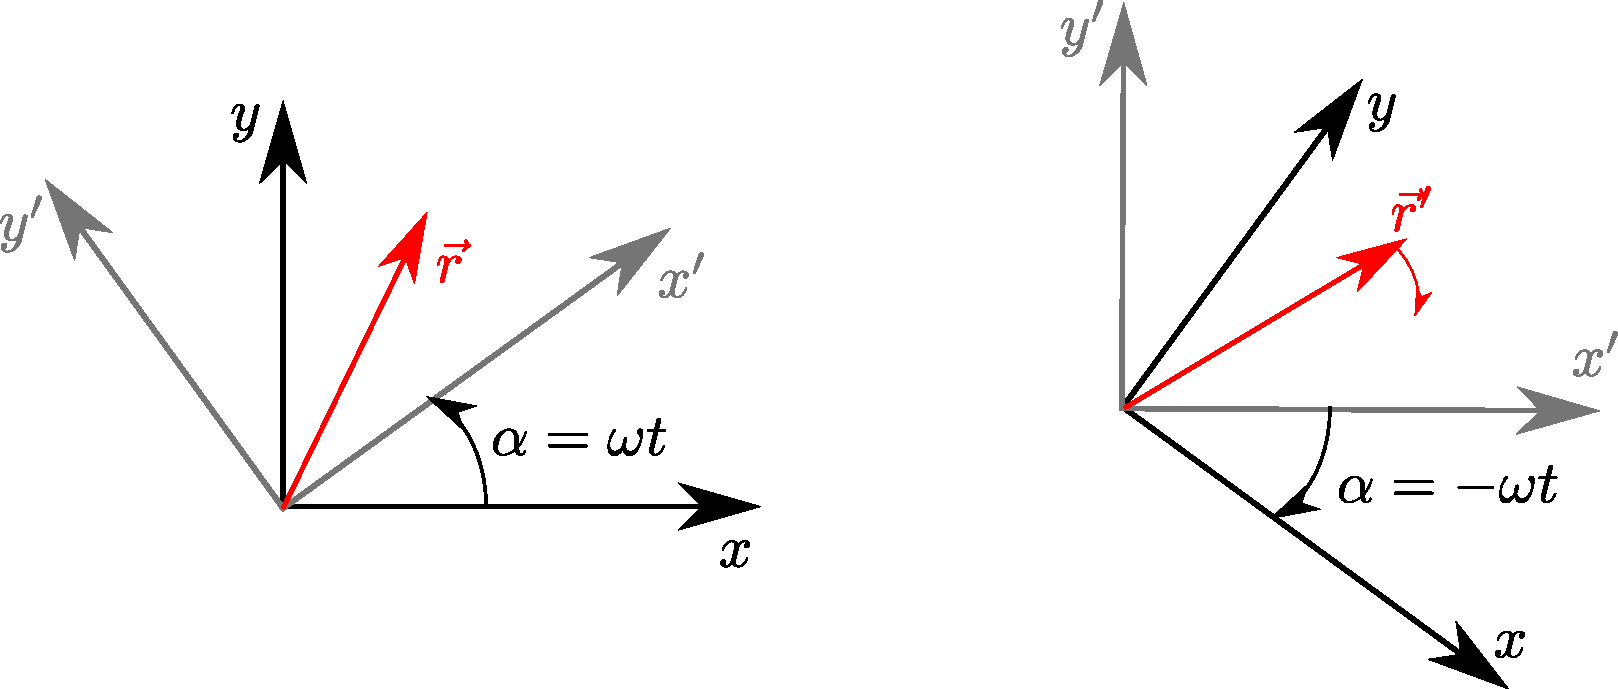
\includegraphics[scale=0.6]{rotating_system.pdf}
\end{figure}
%
If we place ourselves in the rotating frame, we see the system $\Sigma$ rotating \textit{clockwise} with the same angular velocity $\omega$.
%
How do we observe a vector that is described in $\Sigma$ by $\vec{r}$?
%
Let's call our observation $\vec{r}'$ and try to find a relation to $\vec{r}$.
%
Our result must be the vector $\vec{r}$ but rotated by an angle $\alpha=-\omega t$.
%
With some trigonometric relations one can easily show the vector $\vec{r}$ is associated in $\Sigma'$ as
%
\begin{align}
\vec{r}' = R(t) \vec{r} = \begin{pmatrix}
\cos \omega t & \sin \omega t \\
-\sin \omega t & \cos \omega t
\end{pmatrix} \vec{r} =  \begin{pmatrix}
1 & 0 \\
0 & 1
\end{pmatrix} \vec{r} \cos \omega t + \begin{pmatrix}
0 & 1 \\
-1 & 0
\end{pmatrix} \vec{r} \sin \omega t .
\end{align}
%
If we define  
\begin{align}
I =  \begin{pmatrix}
0 & 1 \\
-1 & 0
\end{pmatrix}  , \qquad \boldsymbol{1} = \begin{pmatrix}
1 & 0 \\
0 & 1
\end{pmatrix}
\end{align} 
%
we can compactly write 
%
\begin{align}
R(t) = \boldsymbol{1} \cos \omega t + I \sin \omega t .
\end{align}
%
One can easily show that $I^2 = - \boldsymbol{1}$.
%
Does this look familiar? Yes, it looks like the imaginary unit $\mathrm{i}$ and like the Euler formula for complex numbers one can write the rotation matrix in polar form as a \textit{matrix exponential} 
%
\begin{align}
R(t) = \boldsymbol{1} \cos \omega t + I \sin \omega t = \e^{I\alpha} .
\end{align}

%
We can now write
%
\begin{align}
\boxed{\vec{r}' = R(t) \vec{r} =  \e^{I \omega t}  \vec{r} \iff \vec{r} = \e^{-I \omega t}  \vec{r}' =R(-t) \vec{r}'  .}
\end{align}

Having this relation at hand we can find expressions how a vector changes in the rotating system.
%
Let's us begin with describing how a change of $\vec{r}$ is measured into $\Sigma'$, i.e.
%
\begin{align}
\frac{\d \vec{r}}{\d t} = \frac{\d R(-t)}{\d t} \vec{r}' + R(-t) \frac{\d \vec{r}'}{\d t} =   -\omega I  R(-t) \vec{r}' + R(-t) \frac{\d \vec{r}'}{\d t} ,
\end{align}
%
where we have used the differentiation rule for an exponential to get
%
\begin{align}
\frac{\d R(t)}{\d t} = \omega I  \e^{I \omega t} = \omega I R(t).
\end{align}
%
We can identify $\vec{u}' = {\d \vec{r}'}/{\d t}$ as the velocity measured in $\Sigma'$, thus
%
\begin{align}
\frac{\d \vec{r}}{\d t} =  -\omega I R(-t) \vec{r}' + R(-t) \vec{u}'.
\end{align}

As the next step we consider the second time derivative in the inertial system, i.e.
%
\begin{align}
\frac{\d^2 \vec{r}}{\d^2 t} & = \frac{\d}{\d t} \left( - \omega I  R(-t) \vec{r}' + R(-t) \vec{u}' \right) \\
&= \omega I \omega I R(-t) \vec{r}' - 2 \omega I R(-t) \vec{u}' + R(-t)  \frac{\d^2 \vec{r}'}{\d t^2} .
\end{align}
%
We know that in the inertial system $\Sigma$ Newton's second law is valid and hence ${\d^2 \vec{r}}/{\d t^2}=\vec{F}/m$, where $\vec{F}$ is the force that is measured in $\Sigma$.
%
By multiplying the rotation matrix $R(t)$ from the left we obtain the force $\vec{F'}$ that we measure in the rotation system.
%
Consequently, we get after solving for ${\d^2 \vec{r}'}/{\d t^2}$ 
%
\begin{align}
\boxed{
\frac{\d^2 \vec{r}'}{\d^2 t} = \frac{\vec{F}'}{m}-  \omega I \omega I \vec{r}' + 2  \omega I \vec{u}' ,
}
\end{align}
%
which are the equations of motion that are valid in a system that is rotating anti-clockwise with angular velocity $\omega$ relative to an inertial system.
%
It says that additionally to the physical forces $\vec{F}'$ we measure, we have to take into account \textit{apparent} forces that stem only from relative rotation and not from fundamental interactions.
%
Note that component-wise we have
%
\begin{align}
\frac{\d^2 x'}{\d t^2} = F'_x/m + \omega^2 x' +  \omega u'_y \\
\frac{\d^2 y'}{\d t^2} = F'_x/m + \omega^2 y' -\omega u'_x,
\end{align}
%
where the terms linear in $\omega$ are identical to the $x$ and $y$ components of the 3D cross product
%
\begin{align}
-\begin{pmatrix}
0 \\
0 \\
\omega
\end{pmatrix} \times
\begin{pmatrix}
u'_x \\
u'_y \\
0
\end{pmatrix} = 
\begin{pmatrix}
\omega u'_y \\
-\omega u_x' \\
0
\end{pmatrix}.
\end{align}
%
Thus the action of the matrix $\omega I$ on a 2D vector can be seen as an analogue to the action of taking the cross product $-\vec{\omega} \times$ in three dimensions.
%
Thus we can invent the notation $\omega \times := -\omega I$ in 2D and write 
%
\begin{align}
\boxed{
\frac{\d^2 \vec{r}'}{\d^2 t} = \frac{\vec{F}'}{m} - \omega \times (\omega \times \vec{r}') - 2  \omega \times \vec{u}' ,
}
\end{align}

\section{From particle to field equations}

\subsection{The continuous limit}

Collecting all the forces considered above we can write down the equations of motion for a fluid parcel in a rotating system as
%
\begin{align}
\frac{\d^2 \vec{r}}{\d^2 t} = \frac{\d \vec{u}}{\d t} = \frac{\vec{f}^b(\vec{r},t)}{\rho(\vec{r},t)} -\frac{1}{\rho(\vec{r},t)} \nabla p(\vec{r}, t)+ \frac{\nu}{\rho(\vec{r}, t)} \Laplace \vec{u}(\vec{r}, t) -  \omega \times (\omega \times \vec{r}) - 2 \omega \times \vec{u}
\end{align}
%
Until here, we understood the vector $\vec{r}$ as the position of the parcel at time $t$, so actually $\vec{r}=\vec{r}(t)$ and so $\rho(\vec{r},t)=\rho(\vec{r}(t),t)$ and $\vec{u}(\vec{r},t)=\vec{u}(\vec{r}(t),t)$.
%
Also the time derivative $\d / \d t$ means that the change is considered at the position of the fluid parcel.
%
This perspective on the dynamics is also called the \textit{Lagrangian point of view}.
%
However, when we want to describe a fluid efficiently we do not want to follow each parcel individually.
%
We are more interested in how the \textit{field} changes at a particular point in space, which is also closer to our way of observing the fluid.
%
Thus, instead of describing the set of parcels by $\left\{ \rho(\vec{r}(t), t), \vec{u}(\vec{r}(t), t)\right\}$ we are interested in the fields $\rho(\vec{r},t), \vec{u}(\vec{r},t)$ as \textit{continuous} functions of time and space.
%
This point of view is referred to as the \textit{Eulerian} one.

But how is now the change $\d / \d t$ at the fluids parcel related to the change observed at a fixed position, i.e. $\partial / \partial t$?
%
In order to find out we just consider the time derivative $\d / \d t$ of for instance $\rho$ and write out everything explicitly, i.e.
%
\begin{align}
\frac{\d \rho(\vec{r}(t), t)}{\d t} = ?
\end{align}
%
We can identify an application of the chain rule and write
%
\begin{align}
\frac{\d \rho(\vec{r}(t), t)}{\d t} & = \frac{\d \vec{r}(t)}{\d t} \cdot \left . \nabla \rho(\vec{r}, t)\right |_{\vec{r} = \vec{r}(t)} + \left .\frac{\partial \rho(\vec{r}, t)}{ \partial t} \right |_{\vec{r} = \vec{r}(t)} \\
& = \vec{u}(\vec{r}(t),t) \cdot \left . \nabla \rho(\vec{r}, t)\right |_{\vec{r} = \vec{r}(t)} + \left .\frac{\partial \rho(\vec{r}, t)}{ \partial t} \right |_{\vec{r} = \vec{r}(t)} \\
& = \left . \left(  \vec{u}(\vec{r},t) \cdot  \nabla \rho(\vec{r}, t) + \frac{\partial \rho(\vec{r}, t)}{ \partial t} \right) \right |_{\vec{r} = \vec{r}(t)}
\end{align}
%
We can now fix our point of observation $\vec{r}$ if we say that this location is the location of some parcel moving along $\vec{r}(t)$ at time $t$.
%
Since our fluid is continuous, there is always a parcel passing the point $\vec{r}$ at time $t$.
%
Thus we can write
%
\begin{align}
\frac{\d \rho(\vec{r}, t)}{\d t} = \vec{u}(\vec{r},t) \cdot  \nabla \rho(\vec{r}, t) + \frac{\partial \rho(\vec{r}, t)}{ \partial t}
\end{align}
%
This means that the \textit{total change} of the quantity $\rho$ at position $\vec{r}$ and time $t$ is given by the variation of $\rho$ that is \textit{independent of the fluid flow} and the change that happens due to the flow passing by, i.e. the \textit{advection}.

Finally we can write the so-called Navier-Stokes equation in the Eulerian frame as
%
\begin{align}
\boxed{
 \frac{\partial \vec{u}(\vec{r},t)}{\partial t} = - (\vec{u}(\vec{r}, t)\cdot \nabla) \vec{u}(\vec{r}, t) +  \frac{\vec{f}^b(\vec{r},t)}{\rho(\vec{r},t)} -\frac{1}{\rho(\vec{r},t)} \nabla p(\vec{r}, t)+ \frac{\nu}{\rho(\vec{r}, t)} \Laplace \vec{u}(\vec{r}, t) -  \omega \times (\omega \times \vec{r}) - 2 \omega \times \vec{u} 
}.
\end{align}
%

\subsection{The continuity equation}


We see from the Navier-Stokes equation above that we are lacking some information.
%
The density $\rho(\vec{r}, t)$ as well as the pressure field are not determined from the equation of motion for the velocity field.
%
Thus we have to extend the equation using other laws of physics than Newton's second law.
%
For the density such an equation can be found by considering the \textit{conservation of mass}.
%
\begin{figure}[H]
\begin{center}
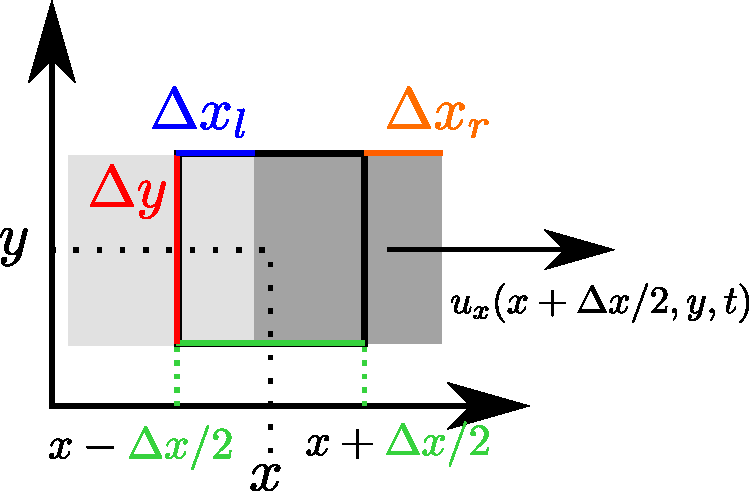
\includegraphics[scale=0.7]{continuity.pdf}
\end{center}
\end{figure}

The mass $\overline{\Delta m}(x,y,t)$ in a \textit{fixed} frame centered at $x,y$ (different from the mass $\Delta m$ of the moving parcel!) can only change, if mass is entering or leaving the frame over a time interval $\Delta t$.
%
If we consider the figure and we restrict ourselves to a flow that has only an $x$-component, the mass $\Delta m_+$ that is entering the frame from the left is
%
\begin{align}
\Delta m_+ = \rho(x-\Delta x/2, y, t) \Delta x_l \Delta y
\end{align}
%
and the mass $\Delta m_-$ that is leaving the frame on the right is
\begin{align}
\Delta m_- = \rho(x+\Delta x/2, y, t) \Delta x_r \Delta y
\end{align}
%
According to the conservation of mass, the total change of mass would then be $\overline{\Delta m}(x,y,t+\Delta t) - \overline{\Delta m}(x,y,t) = \Delta m_+ - \Delta m_- $.
%
Now we can further evaluate the appearing quantities.
%
First, $\Delta x_l$ is the distance the fluid travels within the small time $\Delta t$, thus
$\Delta x_l = u_x(x-\Delta x/2,y,t) \Delta t$.
%
Second, $\Delta x_r$ can determined likewise but with the velocity that is present on the left side of the box, thus $\Delta x_r = u_x(x+\Delta x/2,y,t) \Delta t$.
%
We can now write the conservation of mass as 
\begin{align}
 \overline{\Delta m}(x,y,t+\Delta t) & - \overline{\Delta m}(x,y,t) = \\ \nonumber
& \rho(x-\Delta x/2, y, t)  u_x(x-\Delta x/2,y,t) \Delta t \Delta y - \rho(x+\Delta x/2, y, t) u_x(x+\Delta x/2,y,t) \Delta t \Delta y
\end{align}
%
On the other hand, since our cell is considered in the Eulerian frame, the extensions $\Delta x \times \Delta y$ is constant, a change in mass is due to a change in the density of that cell, i.e.
%
\begin{align}
\overline{\Delta m}(x,y,t+\Delta t) - \overline{\Delta m}(x,y,t) = (\rho(x,y,t+\Delta t) - \rho(x,y,t))  \Delta x \Delta y
\end{align}
%
If we bring now the last two equations together and rearrange a little bit we get
%
\begin{align}
\frac{\rho(x,y,t+\Delta t) - \rho(x,y,t)}{\Delta t} = -\frac{\rho(x+\Delta x/2, y, t)  u_x(x+\Delta x/2,y,t)- \rho(x-\Delta x/2, y, t) u_x(x-\Delta x/2,y,t)}{\Delta x}  
\end{align}
%
If we now shrink our time interval and the observed cell further and further, we recognize the definition of the partial derivative with respect $x$ and the \textit{partial} derivative with respect to time (since $x,y$ are now constant) and we obtain
%
\begin{align}
\frac{\partial \rho(x,y,t)}{\partial t} = -\frac{\partial [\rho(x, y, t)  u_x(x,y,t)]}{\partial x}  
\end{align}
%
If we would repeat this consideration for the $y$ direction we would obtain the same but with differentiating with respect to $y$.
%
The total contribution to the mass change would then be the sum of the two individual contributions, i.e.
%
\begin{align}
\frac{\partial \rho(x,y,t)}{\partial t} = -\frac{\partial [\rho(x, y, t)  u_x(x,y,t)]}{\partial x} - \frac{\partial [\rho(x, y, t)  u_y(x,y,t)]}{\partial y}  
\end{align}
%
Switching to the vector notation we get the famous \textit{mass continuity equation}
%
\begin{align}
\frac{\partial \rho(\vec{r},t)}{\partial t} = -\mathrm{div} [ \rho(\vec{r}, t)  \vec{u}(\vec{r},t)],
\end{align}
%
where the divergence of a vector field $\vec{v}$ is a scalar field and it is defined as $\mathrm{div} \vec{v} = \sum_k \partial v_k / \partial x_k $.

We are now able to extend the Navier-Stokes equation by the continuity equation and have an equation of motion for the density
%
\begin{empheq}[box=\widefbox]{align}
 \frac{\partial \vec{u}(\vec{r},t)}{\partial t} & = - (\vec{u}(\vec{r}, t)\cdot \nabla) \vec{u}(\vec{r}, t) +  \frac{\vec{f}^b(\vec{r},t)}{\rho(\vec{r},t)} -\frac{1}{\rho(\vec{r},t)} \nabla p(\vec{r}, t)+ \frac{\nu}{\rho(\vec{r}, t)} \Laplace \vec{u}(\vec{r}, t) -  \omega \times (\omega \times \vec{r}) - 2 \omega \times \vec{u} \\
 \frac{\partial \rho(\vec{r},t)}{\partial t} & = -\mathrm{div} [ \rho(\vec{r}, t)  \vec{u}(\vec{r},t)].
\end{empheq}
%
\end{document}